%%%%%%%%%%%%%%%%%%%%%%%%%%%%%%%%%%%%%%%%%
% Beamer Presentation
% LaTeX Template
% Version 1.0 (10/11/12)
%
% This template has been downloaded from:
% http://www.LaTeXTemplates.com
%
% License:
% CC BY-NC-SA 3.0 (http://creativecommons.org/licenses/by-nc-sa/3.0/)
%
%%%%%%%%%%%%%%%%%%%%%%%%%%%%%%%%%%%%%%%%%

%----------------------------------------------------------------------------------------
%	PACKAGES AND THEMES
%----------------------------------------------------------------------------------------

\documentclass{beamer}

\mode<presentation> {

% The Beamer class comes with a number of default slide themes
% which change the colors and layouts of slides. Below this is a list
% of all the themes, uncomment each in turn to see what they look like.

%\usetheme{default}
%\usetheme{AnnArbor}
%\usetheme{Antibes}
%\usetheme{Bergen}
%\usetheme{Berkeley}
\usetheme{Berlin}
%\usetheme{Boadilla}
%\usetheme{CambridgeUS}
%\usetheme{Copenhagen}
%\usetheme{Darmstadt}
%\usetheme{Dresden}
%\usetheme{Frankfurt}
%\usetheme{Goettingen}
%\usetheme{Hannover}
%\usetheme{Ilmenau}
%\usetheme{JuanLesPins}
%\usetheme{Luebeck}
%\usetheme{Madrid}
%\usetheme{Malmoe}
%\usetheme{Marburg}
%\usetheme{Montpellier}
%\usetheme{PaloAlto}
%\usetheme{Pittsburgh}
%\usetheme{Rochester}
%\usetheme{Singapore}
%\usetheme{Szeged}
%\usetheme{Warsaw}

% As well as themes, the Beamer class has a number of color themes
% for any slide theme. Uncomment each of these in turn to see how it
% changes the colors of your current slide theme.

%\usecolortheme{albatross}
%\usecolortheme{beaver}
%\usecolortheme{beetle}
%\usecolortheme{crane}
%\usecolortheme{dolphin}
%\usecolortheme{dove}
%\usecolortheme{fly}
%\usecolortheme{lily}
%\usecolortheme{orchid}
%\usecolortheme{rose}
%\usecolortheme{seagull}
%\usecolortheme{seahorse}
%\usecolortheme{whale}
%\usecolortheme{wolverine}

%\setbeamertemplate{footline} % To remove the footer line in all slides uncomment this line
%\setbeamertemplate{footline}[frame number] % To replace the footer line in all slides with a simple slide count uncomment this line

\setbeamertemplate{navigation symbols}{} % To remove the navigation symbols from the bottom of all slides uncomment this line
}

\usepackage{graphicx} % Allows including images
\usepackage{booktabs} % Allows the use of \toprule, \midrule and \bottomrule in tables
\usepackage[english]{babel}
\usepackage{csquotes}
\usepackage[utf8]{inputenc}
\usepackage{amsmath}
\usepackage{amsfonts}
\usepackage{pdfpages}
\usepackage{textpos}

\usepackage{amsthm}
\usepackage{setspace}

\usepackage[authordate,backend=biber]{biblatex-chicago}
\addbibresource{biblio.bib}

\graphicspath{ {img/} }

%----------------------------------------------------------------------------------------
%	TITLE PAGE
%----------------------------------------------------------------------------------------

\title[Bachelorarbeit in Informatik: Solving the DARP with the Firefly Metaheuristic]{Solving the Dial-a-Ride Problem with the Firefly Metaheuristic} % The short title appears at the bottom of every slide, the full title is only on the title page

\author[Fernando Bombardelli da Silva]{Fernando Bombardelli da Silva} % Your name
\institute[Technische Universität Berlin] % Your institution as it will appear on the bottom of every slide, may be shorthand to save space
{
Technische Universität Berlin \\ % Your institution for the title page
Fakultät IV Elektrotechnik und Informatik \\
Bachelorstudiengang Informatik \\
\medskip
\textbf{Bachelorarbeit} \\
\textbf{Advisor: Dr.-Ing. Axel Heßler}\\
\medskip
\textit{bombardelli.f@gmail.com} % Your email address
}
\date{Berlin, 21st March 2016} % Date, can be changed to a custom date

\begin{document}

\begin{frame}
\titlepage % Print the title page as the first slide
\end{frame}

\begin{frame}
\frametitle{Contents} % Table of contents slide, comment this block out to remove it
\tableofcontents % Throughout your presentation, if you choose to use \section{} and \subsection{} commands, these will automatically be printed on this slide as an overview of your presentation
\end{frame}

%----------------------------------------------------------------------------------------
%	PRESENTATION SLIDES
%----------------------------------------------------------------------------------------

%------------------------------------------------
\section{Introduction} % Sections can be created in order to organize your presentation into discrete blocks, all sections and subsections are automatically printed in the table of contents as an overview of the talk
%------------------------------------------------

%\subsection{Subsection Example} % A subsection can be created just before a set of slides with a common theme to further break down your presentation into chunks
\subsection{Overview}

\begin{frame}
\frametitle{Introduction \& Motivation}
\begin{itemize}
\item The DARP: A vehicle routing problem characterized by
	\begin{itemize}
	\item User-orientation
	\item Small vehicles, like vans, shared by users
	\item Flexible routes and schedules
	\end{itemize}
\item In Germany: (An-)Rufbus or Taxibus. In Switzerland: Publicar
\item Example of application: Patients of hemodialysis
\item Their need: Door-to-door transport from home to the hospital
\pause
\item \textbf{Motivations:}
	\begin{itemize}
	\item Improvement of urban mobility and public transportation
	\item Reduction of costs for people who need this kind of transport
	\end{itemize}
\end{itemize}
\end{frame}

\begin{frame}
\frametitle{Approach \& Contribution}
\begin{itemize}
\item Problem of optimization of the operation costs
\item Subject to a set of constraints that guarantee comfort
\pause
\item We proceed with 2 approaches:
	\begin{itemize}
	\item Exact approach with a generic solver
	\item Near-optimal approach with the implementation of a metaheuristic
	\end{itemize}
\pause
\item Our contribution:
	\begin{itemize}
	\item Comparison of the generic solver with the metaheuristic
	\item Application of swarm intelligence to the DARP
	\item New way to represent the solution
	\end{itemize}
\end{itemize}
\end{frame}

%------------------------------------------------
% Definition
\subsection{Definition}
%------------------------------------------------

\begin{frame}
\frametitle{The Dial-a-Ride Problem (DARP)}
\begin{itemize}
\item The DARP is a vehicle routing problem, proven to be $\mathcal{NP}$-hard
\item It \enquote{extends} the \emph{Pickup and Deliver Vehicle Routing Problem} and the \emph{Vehicle Routing Problem with Time Windows}
\pause
\item There is a fleet of \textbf{homogeneous vehicles} with a \textbf{unique depot}
\item Set of transport requests from passengers, known beforehand (\textbf{static} version)
\item Maximal vehicle route duration and vehicle capacity
\item Maximal user ride time
\end{itemize}
\end{frame}

\begin{frame}
\frametitle{Request Characteristics}
\begin{itemize}
\item Pick-up and drop-off locations (ordered pairs)
\item Time windows for the pick-up and for the drop-off
\item Time necessary for boarding or alighting
\item Quantity of passengers
\pause
\item The requests form a full graph G=(V,A), where
	\begin{itemize}
	\item V is the set with every location of every request
	\item A is the set of edges that tell the travel costs and travel times between any pair of locations
	\end{itemize}
\pause
\item The costs and time are assumed to be the \emph{Euclidean distance} between the locations
\end{itemize}
\end{frame}

\begin{frame}
\frametitle{Goal}
\begin{definition}[Route]
The order of the locations through which a vehicle travels. It always starts and ends at the depot.
\end{definition}
\pause
\begin{definition}[Feasible Solution]
\begin{itemize}
\item Assignment of every request to one, and only one, vehicle
\item Determination of the route of every vehicle
\item Every constraint must be fulfilled
\end{itemize}
\end{definition}
\pause
\textbf{Optimal Solution:} Feasible solution whose total duration time is less than or equal to any other feasible solution's total duration time

\end{frame}

%------------------------------------------------
% Theoretical Framework
\section{Development}
\subsection{Theoretical Framework}
%------------------------------------------------

\begin{frame}
\frametitle{Exact Approach}
\begin{itemize}
\item \textbf{Integer Linear Programming}
\item Method commonly used in mathematics and operations research
\item Represent the problem in a mathematical language (e.g. \emph{AMPL})
\item Solve via generic solver (e.g. \emph{GNU Linear Programming Kit})
\item Algorithms behind it: \emph{Simplex}, \emph{branch and bound}, \emph{cutting plane}
\end{itemize}
\end{frame}

\begin{frame}
\frametitle{Near-optimal Approach}
\begin{itemize}
\item Implement a metaheuristic named \textbf{Firefly Algorithm (FA)}
\item Other examples: \emph{Simulated annealing}, \emph{genetic algorithms}
\item The FA is nature-inspired and applies the concept of swarm intelligence
\item Similar to: \emph{Ant colony}, \emph{particle swarm optimization}
\pause
\item Represent the position of a firefly as a vector
\item Represent a solution as a firefly (i.e. the vector of its position)
\end{itemize}
\end{frame}

\begin{frame}
\frametitle{Near-optimal Approach}
\begin{itemize}
\item Simulate the movements of the insects, based on 3 rules:
\pause
\item Fireflies are attracted to each other regardless of their sex
\pause
\item The better the solution represented by a firefly, the brighter is its emitted light
\pause
\item The attractiveness of a firefly $\mathbf{x}$ to another one $\mathbf{y}$ is directly proportional to the brightness of $\mathbf{y}$ and inversely proportional to the distance between them
\pause
\item \textbf{Result:} Ideally, there will be a convergence of fireflies to the optimum
\end{itemize}
\end{frame}

%------------------------------------------------
% Designing the Firefly Metaheuristic
\subsection{Designing the Firefly Metaheuristic}
%------------------------------------------------

\begin{frame}
\frametitle{Solution Representation}
\begin{itemize}
\item $\mathbf{v} = (v_1, v_2,...,v_{k+1})$, where $v_1,v_2,...,v_{k+1} \in \mathbb{N}_{\geq0}$ and $k$ is the number of vehicles
\item Initial solution easily generated, simply random numbers in an interval
\pause
\item A value in $v_1$ represents a unique assignment from requests to vehicles, it may vary between $0$ and $k^n$, where $n$ is the number of requests
\end{itemize}
\end{frame}

\begin{frame}
\frametitle{Solution Representation}
\begin{itemize}
\item The values in $v_2,...,v_{k+1}$ represent each vehicle's routes, analogously to $v_1$
\item The possible arrangement of the requests can be seen as a tree
\end{itemize}
\begin{figure}[b]
\centering
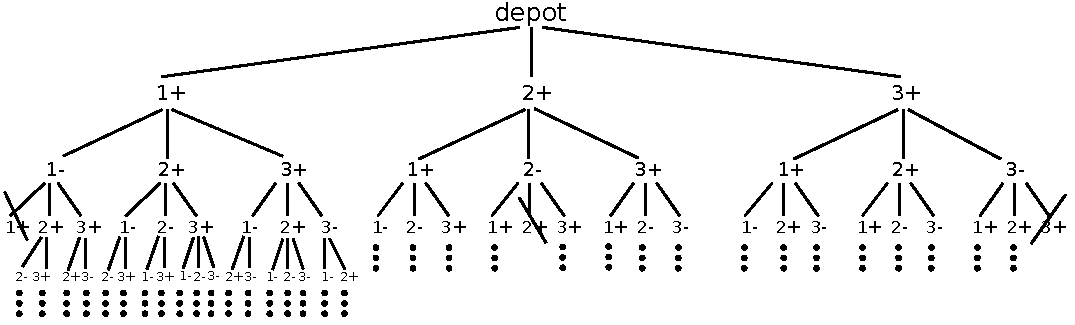
\includegraphics[width=\textwidth]{fig_tree_bus_route}
\end{figure}
\end{frame}

\begin{frame}
\frametitle{Correction of Unfeasibility}
\begin{itemize}
\item Time constraints cause unfeasibilty of solutions
\item Fireflies in these unfeasible regions should be moved into a feasible one
\item Constraint satisfaction problem + Arc Consistency \#3
\end{itemize}
\begin{figure}[b]
\centering
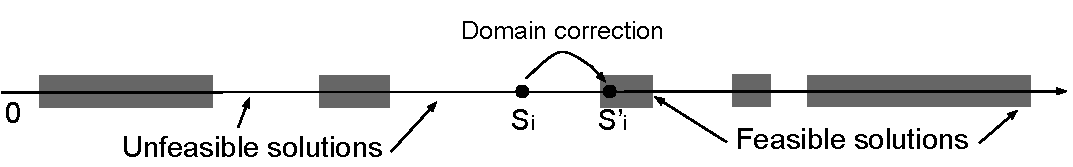
\includegraphics[width=\textwidth]{fig_solution_domain}
\end{figure}
\end{frame}

%------------------------------------------------
% Evaluation
\section{Conclusion}
\subsection{Evaluation}
%------------------------------------------------
\begin{frame}
\frametitle{Generic Solver vs. Metaheristic}
\begin{itemize}
\item CPU: Intel Xeon 2.3 GHz 64bits, 15GB of RAM, Linux OS
\item Generic solver: GNU Linear Programming Kit.
\item Metaheuristic implemented in Python with SciPy
\item Instances created from an instance of the literature
\end{itemize}
\end{frame}

\begin{frame}
\frametitle{Generic Solver vs. Metaheristic}
\begin{itemize}
\item Solution through GLPK is impracticable. Exponential growth of time
\item Firefly implementation shows a steady growth of CPU time
\end{itemize}
\begin{table}[h]
\centering
\caption{Results of the first evaluation}
\footnotesize
\setstretch{1}
\begin{tabular}{l | r | r | r | r | r | r}
\hline
\textbf{Inst.} & \textbf{Req.} & \textbf{Opt.} & \textbf{CPU-GLPK} & \textbf{Firefly Sol.} & \% \textbf{Opt.} & \textbf{CPU-Firefly}\\
\hline
Test-1 & 	2 & 58.05 & 	0.1 & 	69.75 & 	83.2\% & 	7.4 \\
Test-2 & 	4 & 68.10 & 	0.9 & 	98.51 & 	69.1\% & 	11.7 \\
Test-3 & 	5 & 76.27 & 	2.0 & 	134.29 & 	56.8\% & 	2.5 \\
Test-4 & 	6 & 96.54 & 	45.0 & 	149.32 & 	64.6\% & 	3.3 \\
Test-5 & 	8 & - & 	- & 	158.67 & 	- & 	5.7 \\
\hline
\end{tabular}
\label{tab:evaluation-1}
\end{table}
\end{frame}

\begin{frame}
\frametitle{Metaheristic with Literature Instances}
\begin{itemize}
\item 24 instance from the literature
\item Smaller instances: 90\% of optimality in average
\item Deviation to the initial solution varies considerably
\end{itemize}
\begin{table}[H]
\centering
\caption{Results of the second evaluation $-$ Quality and progress}
\scriptsize
\setstretch{1}
\begin{tabular}{l | r | r | r | r | r}
\hline
Instance & Optimum & Final Sol. & Optimality & Initial Sol. & Dev. to Initial Sol.\\
\hline
a2-16 & 	294.25 & 	312.96 & 	94.02\% & 	335.85 & 	6.81\% \\
a2-20 & 	344.83 & 	373.89 & 	92.23\% & 	427.48 & 	12.54\% \\
a2-24 & 	431.12 & 	442.85 & 	97.35\% & 	496.92 & 	10.88\% \\
a3-18 & 	300.48 & 	347.10 & 	86.57\% & 	374.20 & 	7.24\% \\
a3-24 & 	344.83 & 	409.73 & 	84.16\% & 	456.86 & 	10.32\% \\
a3-30 & 	494.85 & 	614.13 & 	80.58\% & 	615.99 & 	0.30\% \\
a3-36 & 	583.19 & 	- & 	- & 	- & 	- \\
a4-16 & 	282.68 & 	310.84 & 	90.94\% & 	354.54 & 	12.33\% \\
\hline
\end{tabular}
\end{table}
\end{frame}

\begin{frame}
\frametitle{Metaheristic with Literature Instances}
\begin{itemize}
\item Optimality sinks as instance sizes rise
\end{itemize}
\begin{table}[H]
\centering
\caption{Results of the second evaluation $-$ Quality and progress}
\scriptsize
\setstretch{1}
\begin{tabular}{l | r | r | r | r | r}
\hline
Instance & Optimum & Final Sol. & Optimality & Initial Sol. & Dev. to Initial Sol.\\
\hline
a4-24 & 	375.02 & 	481.16 & 	77.94\% & 	567.63 & 	15.23\% \\
a4-32 & 	485.50 & 	639.73 & 	75.89\% & 	665.27 & 	3.84\% \\
a4-40 & 	557.69 & 	780.13 & 	71.49\% & 	841.92 & 	7.34\% \\
a4-48 & 	668.82 & 	956.90 & 	69.89\% & 	1032.38 & 	7.31\% \\
a5-40 & 	498.41 & 	779.32 & 	63.95\% & 	818.14 & 	4.74\% \\
a5-50 & 	686.62 & 	926.23 & 	74.13\% & 	1018.84 & 	9.09\% \\
a5-60 & 	808.42 & 	1195.94 & 	67.60\% & 	1257.38 & 	4.89\% \\
a6-48 & 	604.12 & 	993.08 & 	60.83\% & 	1025.55 & 	3.17\% \\
\hline
\end{tabular}
\end{table}
\end{frame}

\begin{frame}
\frametitle{Metaheristic with Literature Instances}
\begin{itemize}
\item Comparison of CPU times to another two approaches
\item $CPU^1$: Parragh (2011). $CPU^2$: Parragh and Schmid (2013).
\end{itemize}
\begin{table}[H]
\centering
\caption{Results of the second evaluation $-$ Running time}
\scriptsize
\setstretch{1}
\begin{tabular}{l | r | r | r}
\hline
Instance & CPU$^1$ & CPU$^2$ & CPU-Firefly\\
\hline
a2-16 & 	68.2 	& 	0.12 & 	\textbf{63.3} \\
a2-20 & 	133.8 	& 	0.28 & 	160.5 \\
a2-24 & 	187.8 	& 	0.35 & 	419.3 \\
a3-18 & 	45.4 	& 	- & 	\textbf{29.5} \\
a3-24 & 	86.8 	& 	0.29 & 	\textbf{77.4} \\
a3-30 & 	105.6 	& 	0.50 & 	151.2 \\
a3-36 & 	162.6 	& 	0.83 & 	370.6 \\
a4-16 & 	26.0 	& 	- & 	\textbf{14.5} \\
a4-24 & 	50.8 	& 	- & 	\textbf{37.0} \\
a4-32 & 	86.0 		& 	0.55 & 	129.4 \\
a4-40 & 	130.6 	& 	0.78 & 	233.5 \\
a4-48 & 	253.8 	& 	1.62 & 	\textbf{222.3} \\
\hline
\end{tabular}
\end{table}
\end{frame}

%------------------------------------------------
% Conclusion
\subsection{Conclusion}
%------------------------------------------------
\begin{frame}
\frametitle{Conclusion}
\begin{itemize}
\item Solution via generic solver is impracticable
\item Solution via FA can solve much larger instances, though not the largest ones
\item Main issue: The time constraints (time windows and ride time)
\item How to overcome: Rethink solution representation, for example
\item Improve efficiency: Reduce domain corrections and improve transformation functions
\end{itemize}
\end{frame}

\renewcommand*{\bibfont}{\scriptsize}
\setlength\bibitemsep{0pt}
\begin{frame}
\nocite{braekers_exact_2014}
\nocite{cordeau_dial--ride_2007}
\nocite{parragh_introducing_2011}
\nocite{parragh_hybrid_2013}
\nocite{ropke_models_2007}
\nocite{yang_firefly_2013}
\begin{block}{Bibliography}
\printbibliography[heading=none]
\end{block}
\end{frame}
%------------------------------------------------

\begin{frame}[c]
\begin{center}
\Huge Thank you for your attention\\
\huge Questions...
\end{center}
\end{frame}

%----------------------------------------------------------------------------------------

\end{document}